\documentclass[10pt]{article}\usepackage[]{graphicx}\usepackage[]{color}
%% maxwidth is the original width if it is less than linewidth
%% otherwise use linewidth (to make sure the graphics do not exceed the margin)
\makeatletter
\def\maxwidth{ %
  \ifdim\Gin@nat@width>\linewidth
    \linewidth
  \else
    \Gin@nat@width
  \fi
}
\makeatother

\definecolor{fgcolor}{rgb}{0.345, 0.345, 0.345}
\newcommand{\hlnum}[1]{\textcolor[rgb]{0.686,0.059,0.569}{#1}}%
\newcommand{\hlstr}[1]{\textcolor[rgb]{0.192,0.494,0.8}{#1}}%
\newcommand{\hlcom}[1]{\textcolor[rgb]{0.678,0.584,0.686}{\textit{#1}}}%
\newcommand{\hlopt}[1]{\textcolor[rgb]{0,0,0}{#1}}%
\newcommand{\hlstd}[1]{\textcolor[rgb]{0.345,0.345,0.345}{#1}}%
\newcommand{\hlkwa}[1]{\textcolor[rgb]{0.161,0.373,0.58}{\textbf{#1}}}%
\newcommand{\hlkwb}[1]{\textcolor[rgb]{0.69,0.353,0.396}{#1}}%
\newcommand{\hlkwc}[1]{\textcolor[rgb]{0.333,0.667,0.333}{#1}}%
\newcommand{\hlkwd}[1]{\textcolor[rgb]{0.737,0.353,0.396}{\textbf{#1}}}%
\let\hlipl\hlkwb

\usepackage{framed}
\makeatletter
\newenvironment{kframe}{%
 \def\at@end@of@kframe{}%
 \ifinner\ifhmode%
  \def\at@end@of@kframe{\end{minipage}}%
  \begin{minipage}{\columnwidth}%
 \fi\fi%
 \def\FrameCommand##1{\hskip\@totalleftmargin \hskip-\fboxsep
 \colorbox{shadecolor}{##1}\hskip-\fboxsep
     % There is no \\@totalrightmargin, so:
     \hskip-\linewidth \hskip-\@totalleftmargin \hskip\columnwidth}%
 \MakeFramed {\advance\hsize-\width
   \@totalleftmargin\z@ \linewidth\hsize
   \@setminipage}}%
 {\par\unskip\endMakeFramed%
 \at@end@of@kframe}
\makeatother

\definecolor{shadecolor}{rgb}{.97, .97, .97}
\definecolor{messagecolor}{rgb}{0, 0, 0}
\definecolor{warningcolor}{rgb}{1, 0, 1}
\definecolor{errorcolor}{rgb}{1, 0, 0}
\newenvironment{knitrout}{}{} % an empty environment to be redefined in TeX

\usepackage{alltt}

\usepackage{amsmath,amssymb,amsthm}
\usepackage{fancyhdr,url,hyperref}
\usepackage{graphicx,xspace}
\usepackage{subfigure}
\usepackage{tikz}
\usetikzlibrary{arrows,decorations.pathmorphing,backgrounds,positioning,fit,through}

\oddsidemargin 0in  %0.5in
\topmargin     0in
\leftmargin    0in
\rightmargin   0in
\textheight    9in
\textwidth     6in %6in
%\headheight    0in
%\headsep       0in
%\footskip      0.5in

\newtheorem{thm}{Theorem}
\newtheorem{cor}[thm]{Corollary}
\newtheorem{obs}{Observation}
\newtheorem{lemma}{Lemma}
\newtheorem{claim}{Claim}
\newtheorem{definition}{Definition}
\newtheorem{question}{Question}
\newtheorem{answer}{Answer}
\newtheorem{problem}{Problem}
\newtheorem{solution}{Solution}
\newtheorem{conjecture}{Conjecture}

\pagestyle{fancy}

\lhead{\textsc{Prof. McNamara}}
\chead{\textsc{SDS/MTH 220: Lecture notes}}
\lfoot{}
\cfoot{}
%\cfoot{\thepage}
\rfoot{}
\renewcommand{\headrulewidth}{0.2pt}
\renewcommand{\footrulewidth}{0.0pt}

\newcommand{\ans}{\vspace{0.25in}}
\newcommand{\R}{{\sf R}\xspace}
\newcommand{\cmd}[1]{\texttt{#1}}
\newcommand{\Ex}{\mathbb{E}}

\rhead{\textsc{September 20, 2017}}
\IfFileExists{upquote.sty}{\usepackage{upquote}}{}
\begin{document}

\paragraph{Agenda}
\begin{enumerate}
  \itemsep0em
  \item Simple Linear Regression
  \item Residuals
\end{enumerate}


\paragraph{Warmup: Correlation}
An article reported that there was a 0.42 correlation between alcohol consumption and income among adults with a four-year college degree. Is it reasonable to conclude that increasing one's alcohol consumption will increase one's income? Explain why or why not. 

\vspace{1in}

% MMC, 7e, Ex. 2.59
A college newspaper interviews a psychologist about student ratings of the teaching of faculty members. The psychologist says, ``The evidence indicates that the correlation between the research productivity and teaching rating of faculty members is close to zero." The paper reports this as ``Prof. McDaniel said that good researchers tend to be poor teachers, and vice versa." Explain why the paper's report is wrong. Write a statement in plain language (don't use the word \emph{correlation}) to explain the psychologist's meaning. 

\vspace{1in}

\paragraph{Simple linear regression}
Linear regression can help us understand changes in a numerical response variable in terms of a numerical explanatory variable. 

A simple linear regression model for $y$ in terms of $x$ takes the form
$$
  y_i = \beta_0 + \beta_1 \cdot x_i + \epsilon_i \,, \text{ for } i=1,\ldots,n
$$
\begin{itemize}
  \itemsep0in
  \item $\beta_0$ is the \emph{intercept} and $\beta_1$ is the \emph{slope} coefficient. The $\epsilon_i$'s are the \emph{errors}, or \emph{noise}.
  \item There is only one regression line that fits the data best using a least squares criteria. That is, the \emph{ordinary least squares} regression line is unique.
  \item The true values of the unknown parameters $\beta_0$ and $\beta_1$ are estimated by $b_0$ and $b_1$ (or if you prefer, $\hat{\beta}_0$ and $\hat{\beta}_1$)
  \item The \emph{fitted values} are given by 
  $$
    \hat{y}_i = b_0 + b_1 \cdot x_i
  $$
  \item The model almost never fits perfectly, but what is left over is captured by the \emph{residuals} ($e_i = y_i - \hat{y}_i$)

\end{itemize}

\paragraph{Example: RailTrail}

The Pioneer Valley Planning Commission (PVPC) collected data north of Chestnut Street in Florence, MA for ninety days from April 5, 2005 to November 15, 2005. Data collectors set up a laser sensor, with breaks in the laser beam recording when a rail-trail user passed the data collection station. The data is captured in the \cmd{RailTrail} data set.

\begin{knitrout}
\definecolor{shadecolor}{rgb}{0.969, 0.969, 0.969}\color{fgcolor}\begin{kframe}
\begin{alltt}
\hlkwd{require}\hlstd{(mosaic)}
\end{alltt}


{\ttfamily\noindent\color{warningcolor}{\#\# Warning: package 'dplyr' was built under R version 3.4.1}}\begin{alltt}
\hlkwd{data}\hlstd{(RailTrail)}
\end{alltt}
\end{kframe}
\end{knitrout}
\clearpage
\begin{enumerate}
  \itemsep0.6in
  \item Write the code to create a scatterplot [\cmd{qplot()}] for the $volume$ in terms of $avgtemp$
  \item Describe the form, direction, and strength of the relationship
  \vspace{0.6in}
\end{enumerate}

\begin{knitrout}\footnotesize
\definecolor{shadecolor}{rgb}{0.969, 0.969, 0.969}\color{fgcolor}\begin{kframe}
\begin{alltt}
\hlstd{m1} \hlkwb{<-} \hlkwd{lm}\hlstd{(volume}\hlopt{~}\hlstd{avgtemp,} \hlkwc{data}\hlstd{=RailTrail)}
\hlkwd{coef}\hlstd{(m1)}
\end{alltt}
\begin{verbatim}
## (Intercept)     avgtemp 
##    99.60227     4.80205
\end{verbatim}
\end{kframe}
\end{knitrout}
  %\item Compute the correlation coefficient [\cmd{cor()}]
  %\item Fit the linear regression model using \cmd{lm()}
\begin{enumerate}
  \itemsep0.6in
  \item Interpret the coefficients for the \cmd{Intercept} and \cmd{avgtemp} terms
  \vspace{1in}
\end{enumerate}

\paragraph{Model visualization}

Compare the least squares regression line (right) with the average (left).

\begin{knitrout}
\definecolor{shadecolor}{rgb}{0.969, 0.969, 0.969}\color{fgcolor}\begin{kframe}


{\ttfamily\noindent\color{warningcolor}{\#\# Warning: Deprecated: please use `purrr::possibly()` instead}}

{\ttfamily\noindent\color{warningcolor}{\#\# Warning: Deprecated: please use `purrr::possibly()` instead}}

{\ttfamily\noindent\color{warningcolor}{\#\# Warning: Deprecated: please use `purrr::possibly()` instead}}

{\ttfamily\noindent\color{warningcolor}{\#\# Warning: Deprecated: please use `purrr::possibly()` instead}}

{\ttfamily\noindent\color{warningcolor}{\#\# Warning: Deprecated: please use `purrr::possibly()` instead}}

{\ttfamily\noindent\color{warningcolor}{\#\# Warning: Deprecated: please use `purrr::possibly()` instead}}

{\ttfamily\noindent\color{warningcolor}{\#\# Warning: Deprecated: please use `purrr::possibly()` instead}}

{\ttfamily\noindent\color{warningcolor}{\#\# Warning: Deprecated: please use `purrr::possibly()` instead}}

{\ttfamily\noindent\color{warningcolor}{\#\# Warning: Deprecated: please use `purrr::possibly()` instead}}

{\ttfamily\noindent\color{warningcolor}{\#\# Warning: Deprecated: please use `purrr::possibly()` instead}}\end{kframe}
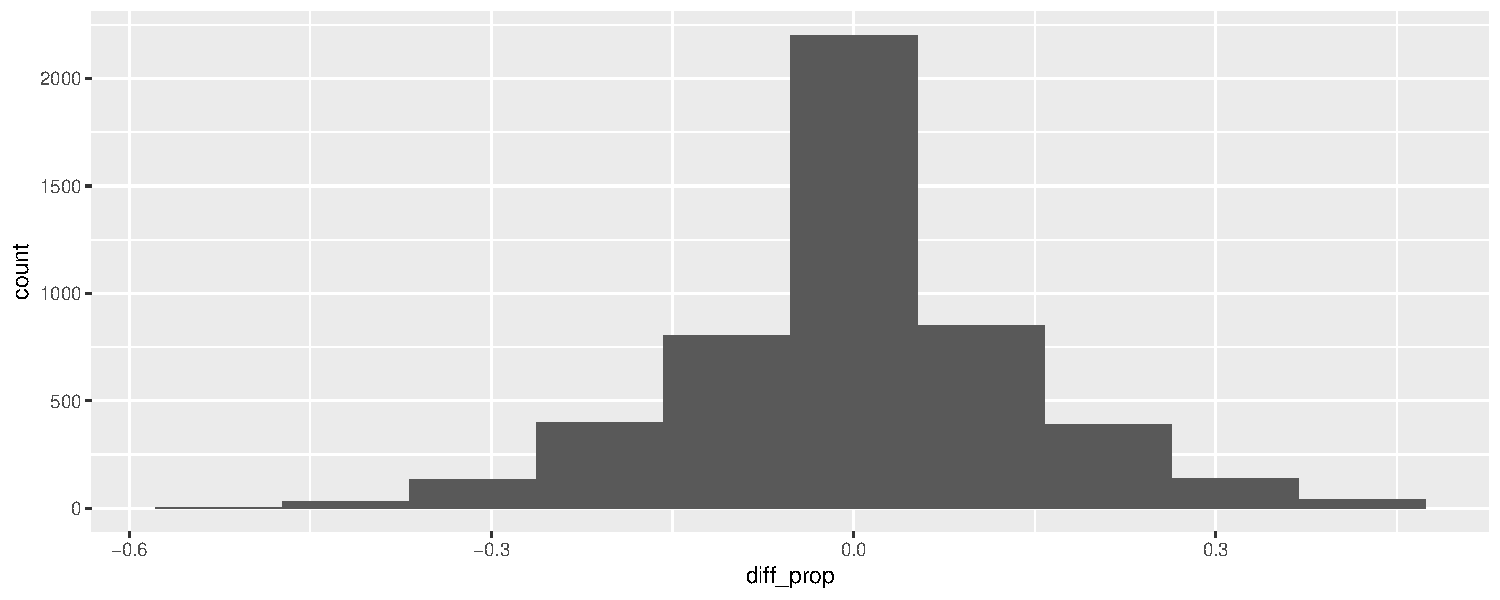
\includegraphics[width=\maxwidth]{figure/unnamed-chunk-3-1} 

\end{knitrout}


\end{document}
